\section{Bound propagation types}
\label{sec:bp_types}

The main goal of this chapter is to explain how we can apply a bound propagation on a Neural Network, made up of only fully connected layers at first, then also ReLU layers. Assume we have a property that set up an upper and lower bound for each neuron of the input. Essentially, let $\textbf{x}$ be the set of input neurons and $x_i$ the i-th neuron of $\textbf{x}$.
We can apply different types of bound propagation. The first that will be dealt with is the \textbf{naive propagation}. 

\subsection{Naive Propagation}

\begin{figure}[t]
	\caption{\label{fig:naive_prop} Example of naive propagation}
	\centering
	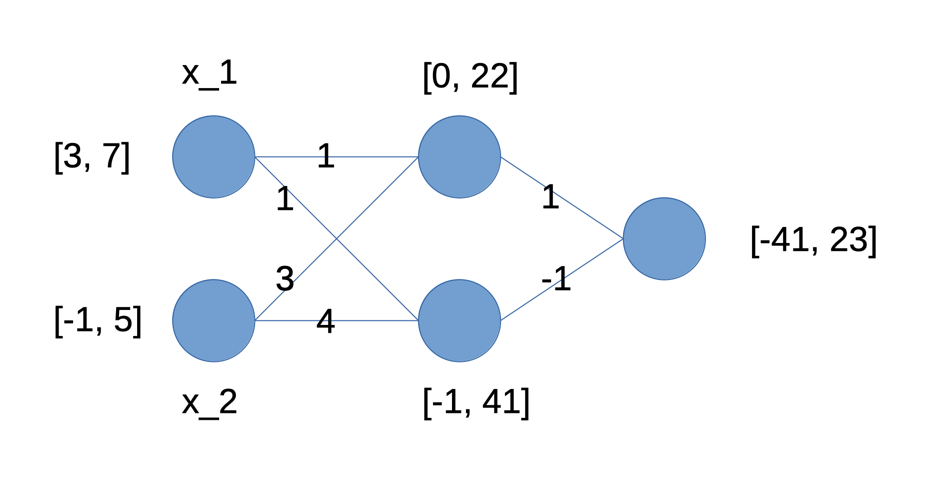
\includegraphics[scale= 0.3]{Chapter5/img/bound-propagation/naive_prop.png}
\end{figure}

In Fig~\ref{fig:naive_prop} represents a neural network consisting of two layers fully connected.\\
By performing the products and sums between the intervals and the fully connected weights along the layers we get an output interval [-41, 23].\\
Let the affine mapping (fc) be defined as  $\textbf{y} = W\textbf{x} + \textbf{b}$
and $W^+$ and $W^-$ be the positive and negative entries of $W$.\\
We also define $l^{+}_i$ and $l^{-}_i$ respectively as the vectors of the upper bounds and of the lower bounds.  

For calculating the intervals of the i-th fully connected layer for all nodes:

\begin{equation}
    \begin{aligned}
        lower\_bound\_i = W^+l^{-}_{i-1} + W^-l^{+}_{i-1} + b\\
        upper\_bound\_i = W^+l^{+}_{i-1} + W^-l^{-}_{i-1} + b
    \end{aligned}
\end{equation}

Now, note that the upper bound 23 of the output cannot be reached. It can appear only if the upper and lower nodes of the hidden layers are respectively 22 and -1 but this is impossible. This is because in order to have 22 in the upper node of the hidden layer it is necessary to have $x_1 = 7$ and $x_2 = 5$ as input values  but to have -1 in the lower node of the hidden layer it is necessary to have $x_1 = 3$ and $x_2 = -1$ at the same time. These two conditions are contradictory and therefore can't be satisfied, this is due to the fact that this is an overestimation of the real bounds. It is also an example of the \textbf{dependency problem}. 
Naive interval analysis suffers from large overestimation errors as it ignores the input dependencies during interval propagation.

\subsection{Symbolic Interval Propagation}
\label{subsec:fc-symbolic-interval-propagation}

\begin{figure}[t]
	\caption{\label{fig:bound_prop}  Example of bound propagation}
	\centering
	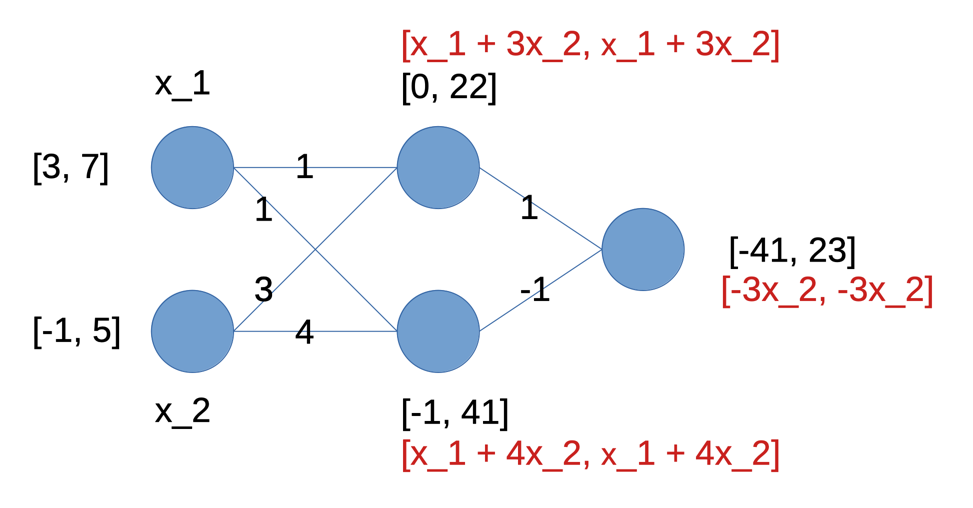
\includegraphics[scale= 0.3]{"Chapter5/img/bound-propagation/bound_prop_2.png"}
\end{figure}

In Fig~\ref{fig:bound_prop}  we use a different approach to overestimate the output interval. The main idea is to minimize overestimation by explicitly representing the intermediate computations of each neuron using symbolic intervals. These intervals encode the interdependency of the inputs and help in accurately estimating the output range of the neuron. In simpler terms, symbolic interval propagation is a technique that optimizes the calculation process within a neuron by using symbolic intervals to better understand the relationships between inputs and reduce the tendency to overestimate the output.\\
This approach on average, reduces significantly the over-approximation error with respect to the naive propagation.

\vspace{10mm}
In our example the intervals, made up respectively from a lower and an  upper bound vector, associated to the nodes of the input layers [$x\_1, x\_2$] are $l^{-}_0 = [3, -1]$ and $l^{+}_0 = [7,5]$.\\
Instead $[x_1 + 3x_2, x_1 + 3x_2]$ and [$x_1 + 4x_2, x_1 + 4x_2$] are the lower and upper symbolic bounds of the intermediate nodes.

Below are the procedure and formulas to compute the symbolic bounds of the i-th layer:
\begin{enumerate}
    \item For the input layer instantiate two identity matrix whose size is the number of input neuron and two zeroes offset vectors. In our example, we would instantiate 2 2x2 matrices and two zero-vectors of 2 elements.

        \begin{equation*}
            lower_0 = \begin{pmatrix}
            1 & 0 & \cdots & 0 \\
            0 & 1 & \cdots & 0 \\
            \vdots & \vdots & \ddots & \vdots \\
            0 & 0 & \cdots & 1
            \end{pmatrix}
        \end{equation*}
        
        \begin{equation*}
            upper_0 = \begin{pmatrix}
            1 & 0 & \cdots & 0 \\
            0 & 1 & \cdots & 0 \\
            \vdots & \vdots & \ddots & \vdots \\
            0 & 0 & \cdots & 1
            \end{pmatrix}
        \end{equation*}

        \begin{equation*}
            lower\_offset_0 = \begin{pmatrix}
            0  \\
            \vdots \\
            0  \\
            \end{pmatrix}
        \end{equation*}

        \begin{equation*}
            upper\_offset_0 = \begin{pmatrix}
            0  \\
            \vdots \\
            0  \\
            \end{pmatrix}
        \end{equation*}
        
    \item
    Let $upper_i$ and $lower_i$ respectively the matrix of the symbolic upper bound equations and lower bound equation of a fully connected layer i.
    A fully connected layer is characterised by a weight matrix $W$ and a bias vector $b$.\\
    Below are the formulas to calculate the upper symbolic bound and the lower symbolic bounds after a fully connected layer:
    \begin{equation}
        \begin{aligned}
            &lower_i = W^+_i lower_{i-1} + W^-_i upper_{i-1}\\
            &upper_i = W^+_i upper_{i-1} + W^-_i lower_{i-1}\\
            &lower\_offset_i = W^+_i lower\_offset_{i-1} + W^-_i upper\_offset_{i-1}\\
            &upper\_offset_i = W^+_i upper\_offset_{i-1} + W^-_i lower\_offset_{i-1}\\
        \end{aligned}
    \end{equation}
    where:\\
    $lower_{i-1}$ and $lower_{i-1}$ are the upper and lower symbolic bounds 
    matrixes of the previous layer. \\

    By iterating the above formula through all layers of a complete fully connected network, you get the symbolic upper and lower bounds equations for each fc layer.

    Given the symbolic upper and lower bounds matrices $lower\_i$, $upper\_i$, $lower\_offset_i$ and $upper\_offset_i$ of layer $i$ and a couple of vectors (the upper and lower bound vector $l^{+}_0$ $l^{-}_0$ ) on the input layer you can calculate the \textbf{numeric} lower and upper bounds of layer $i$. The formulas are below:
    
     \begin{equation}
        \begin{aligned}
            &numeric\_lower_i = lower_{i}^{+} \cdot l^{-}_0 + lower_{i}^{-} \cdot l^{+}_0 + offset_i\\
            &numeric\_upper_i = upper_{i}^{+} \cdot l^{+}_0 + lower_{i}^{-} \cdot l^{-}_0 + offset_i\\
        \end{aligned}
    \end{equation}

    where: \\
     $numeric\_lower_i$ and $numeric\_upper_i$ are the lower and upper numeric bounds vectors of layer $i$\\
     $l^{-}_0$ and $l^{+}_0$ are the lower and upper bounds vectors of input layer\\
\end{enumerate}

By iterating this process for all layers, we get the numeric and numeric bounds for all the layer of the network.\\
The main problem that arises is that we often need to deal with networks formed by FC and ReLU. The rectified linear activation function or ReLU for short is a piecewise linear function that will output the input directly if it is positive, otherwise, it will output zero. But we can't deal with it because it is not a linear and, therefore, we have to use a convex approximation to deal with it.


\subsection{Iterative Refinement Propagation}

\begin{figure}[t]
	\caption{\label{fig:iterative_propagation} Example of bisection and refinement}
	\centering
	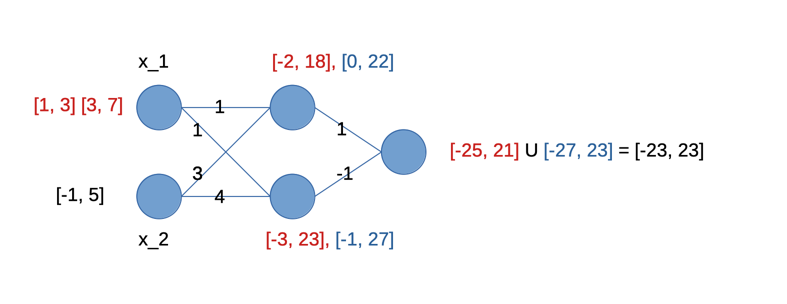
\includegraphics[scale=0.6]{"Chapter5/img/bound-propagation/bisection.png"}
\end{figure}

In fig~\ref{fig:iterative_propagation},  the input interval on a node is divided into two adjacent sub-intervals of equal size, effectively cutting it in half. This division helps decrease the overestimation and allows us to narrow down the range of possible values for the output. As a matter of fact the output interval is tighter respect to the one got with the naive propagation. It's important to note that we can continue refining the output interval by repeatedly splitting the input intervals in order to further tighten the overapproximation. This process is easily parallelizable because each split sub-interval can be independently checked.


    

	

	




